\documentclass{article}
\usepackage[utf8]{inputenc}
\usepackage{hyperref}
\usepackage{color}
\usepackage{tikzsymbols}

\title{Report :: TIPR Assignment - III}
\author{*Put your name here*}
\date{*Put the date here*}

\begin{document}

\maketitle

\section{Configuration}
\begin{itemize}
	\item Python code is written for Python 3. It may not work with Python 2.
	\item The code should be executed from the src folder, otherwise relative paths may not work as expected.
	\item Pass the configuration as a string list. That is, argument should be --filter-config '[8 8 4 4]' (\textbf{with} quotes).
\end{itemize}

\section{Part 1:- Fashion MNIST}
\subsection{Task 1:- Test Model with different number of layers}
Tested model with following architectures:
\begin{itemize}
	\item conv-5-5-32-conv-3-3-64-FCN-500-10
	\item conv-5-5-32-conv-5-5-32-conv-3-3-64-FCN-384-192-10
	\item conv-5-5-64-conv-3-3-64-FCN-384-192-10
\end{itemize}

\begin{figure}[!htb]
	\minipage{0.33\textwidth}
	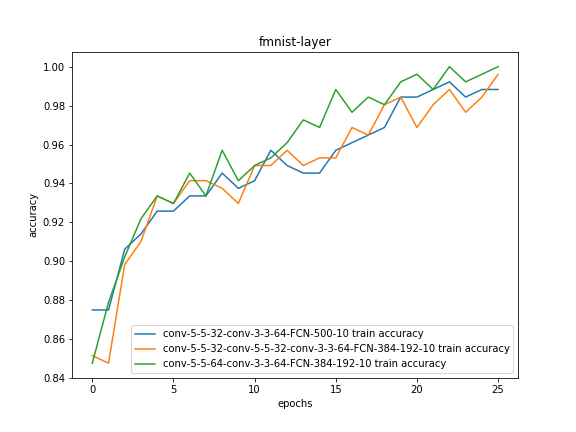
\includegraphics[width=\linewidth]{../output_plots/FMNIST/task-1/fmnist-layer-Accuracy-accuracy.png}
	\caption{Accuracy}\label{fig:part_1_task_1_accuracy}
	\endminipage\hfill
	\minipage{0.33\textwidth}%
	\includegraphics[width=\linewidth]{../output_plots/FMNIST/task-1/fmnist-layer-F1-macro-score-f1-macro.png}
	\caption{F1-Micro}\label{fig:part_1_task_1_f1-micro}
	\endminipage
	\minipage{0.33\textwidth}%
	\includegraphics[width=\linewidth]{../output_plots/FMNIST/task-1/fmnist-layer-F1-micro-score-f1-micro.png}
	\caption{F1-Macro}\label{fig:part_1_task_1_f1-macro}
	\endminipage
\end{figure}

Each plot shows the metric on Y-axis and epochs on X-axis. Different lines in plot corresponds to different models.

\subsection{Task 2:- Test Model with different number of neurons and layers}

Tested model with following configurations:
\begin{itemize}
	\item conv-5-5-64-conv-3-3-64-FCN-512-384-10
	\item conv-7-7-32-conv-5-5-64-FCN-384-192-10
	\item conv-7-7-64-conv-3-3-64-FCN-512-192-10
\end{itemize}

Finally fixed and fine-tuned the 784-50-30-10 model as it took less time for training and had comparable performance.

\begin{figure}[!htb]
	\minipage{0.33\textwidth}
	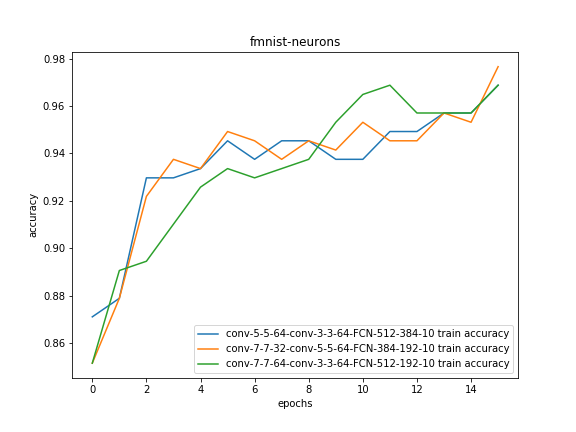
\includegraphics[width=\linewidth]{../output_plots/FMNIST/task-2/fmnist-neurons-Accuracy-accuracy.png}
	\caption{Accuracy}\label{fig:part_1_task_2_accuracy}
	\endminipage\hfill
	\minipage{0.33\textwidth}%
	\includegraphics[width=\linewidth]{../output_plots/FMNIST/task-2/fmnist-neurons-F1-macro-score-f1-macro.png}
	\caption{F1-Micro}\label{fig:part_1_task_2_f1-micro}
	\endminipage
	\minipage{0.33\textwidth}%
	\includegraphics[width=\linewidth]{../output_plots/FMNIST/task-2/fmnist-neurons-F1-micro-score-f1-micro.png}
	\caption{F1-Macro}\label{fig:part_1_task_2_f1-macro}
	\endminipage
\end{figure}

Each plot shows the metric on Y-axis and epochs on X-axis. Different lines in plot corresponds to different models.

\subsection{Task 3:- Test Model with different activation functions}

Tested model with relu, tanh, sigmoid and swish activations functions. The performance of relu and swish were almost same and decided to use swish in the final model.

\begin{figure}[!htb]
	\minipage{0.33\textwidth}
	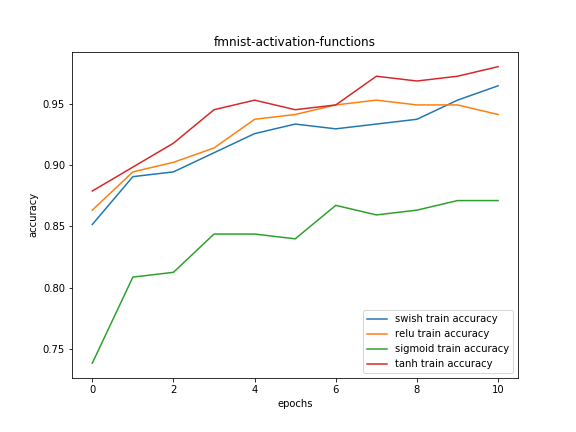
\includegraphics[width=\linewidth]{../output_plots/FMNIST/task-3/fmnist-activation-functions-Accuracy-accuracy.png}
	\caption{Accuracy}\label{fig:part_1_task_3_accuracy}
	\endminipage\hfill
	\minipage{0.33\textwidth}
	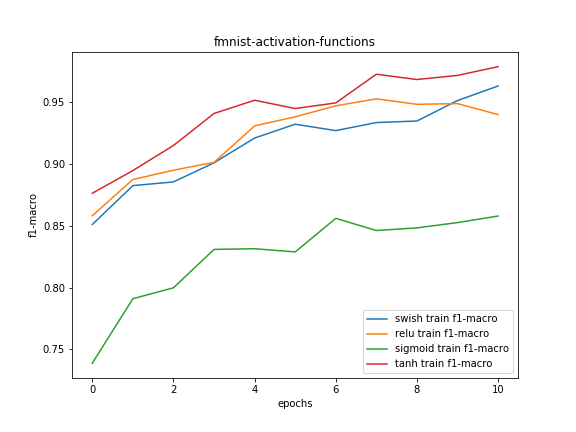
\includegraphics[width=\linewidth]{../output_plots/FMNIST/task-3/fmnist-activation-functions-F1-Macro-score-f1-macro.png}
	\caption{F1-Micro}\label{fig:part_1_task_3_f1-micro}
	\endminipage
	\minipage{0.33\textwidth}
	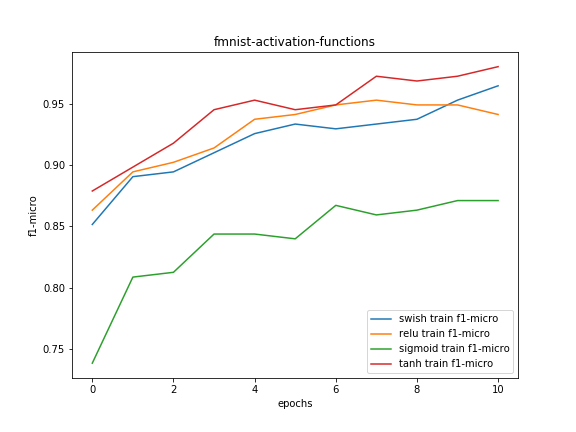
\includegraphics[width=\linewidth]{../output_plots/FMNIST/task-3/fmnist-activation-functions-F1-Micro-score-f1-micro.png}
	\caption{F1-Macro}\label{fig:part_1_task_3_f1-macro}
	\endminipage
\end{figure}

Each plot shows the metric on Y-axis and epochs on X-axis. Different lines in plot corresponds to different models.

\pagebreak
\subsection{Task 4}
After observing above results and trying out various initialization techniques following architecture was finalized:
\begin{enumerate}
	\item Conv1: filter=7x7x1x64, activation=swish
	\item MaxPool1: kernel=2x2, strides=3x3
	\item Conv2: filter=3x3x64x64, activation=swish
	\item MaxPool2: kernel=2x2, strides=3x3
	\item FCN1: output=512, activation=swish
	\item FCN2: output=192, activation=swish
	\item Final output using softmax.
\end{enumerate}

\subsection{Task 5: Semi-supervised learning}
In this task model (selected in Task 4) was trained on 10-50\% of the data and embedding for rest of the images were extracted from the final layer just before the output layer of the network. The images were then clustered according to these embedding into 15 clusters and each cluster was assigned a class label depending on the highest number of images into that cluster belonging to same class.

The final accuracy achieved on validation set after taking 10-50\% of training data in increments of 10\% is as below:
\begin{table}[!htb]
\centering
\begin{tabular}{|c|c|}
	\hline
	Training instances & Accuracy\\
	\hline
	10\% & 88.5\%\\
	20\% & 87.2\%\\
	30\% & 89.4\%\\
	40\% & 88.9\%\\
	50\% & 87.3\%\\
	\hline
\end{tabular}
\end{table}\\

\pagebreak
\subsection{Task 6:- Cluster Projection}
The graphs obtained from above configuration of training instances is as below. These graphs were generated by projecting 1000 randomly selected instances into 2D using t-SNE projection method.

\begin{figure}[!htb]
	\minipage{0.5\textwidth}
	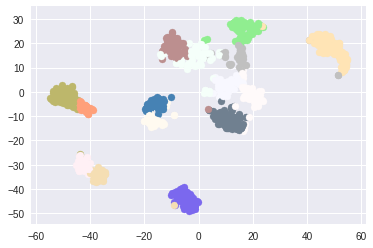
\includegraphics[width=\linewidth]{../output_plots/FMNIST/clustering/cluster-distribution-10.png}
	\caption{10\% training data clusters}\label{fig:part_1_task_5_cluster_10}
	\endminipage\hfill
	\minipage{0.5\textwidth}
	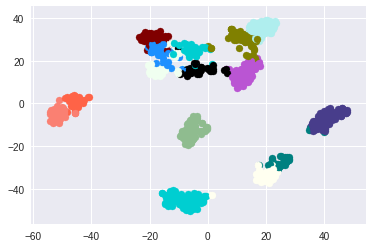
\includegraphics[width=\linewidth]{../output_plots/FMNIST/clustering/cluster-distribution-20.png}
	\caption{20\% training data clusters}\label{fig:part_1_task_5_cluster_20}
	\endminipage\\
	\minipage{0.33\textwidth}
	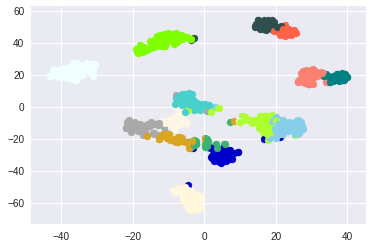
\includegraphics[width=\linewidth]{../output_plots/FMNIST/clustering/cluster-distribution-30.png}
	\caption{30\% training data clusters}\label{fig:part_1_task_5_cluster_30}
	\endminipage\hfill
	\minipage{0.33\textwidth}
	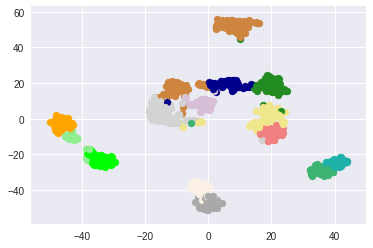
\includegraphics[width=\linewidth]{../output_plots/FMNIST/clustering/cluster-distribution-40.png}
	\caption{40\% training data clusters}\label{fig:part_1_task_5_cluster_40}
	\endminipage
	\minipage{0.33\textwidth}
	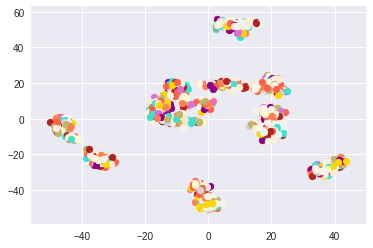
\includegraphics[width=\linewidth]{../output_plots/FMNIST/clustering/cluster-distribution-50.png}
	\caption{50\% training data clusters}\label{fig:part_1_task_5_cluster_50}
	\endminipage
\end{figure}

The corresponding class distribution of points is as below:
\begin{figure}[!htb]
	\minipage{0.5\textwidth}
	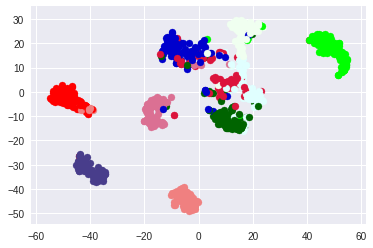
\includegraphics[width=\linewidth]{../output_plots/FMNIST/clustering/class-distribution-10.png}
	\caption{10\% training data classes}\label{fig:part_1_task_5_class_10}
	\endminipage\hfill
	\minipage{0.5\textwidth}
	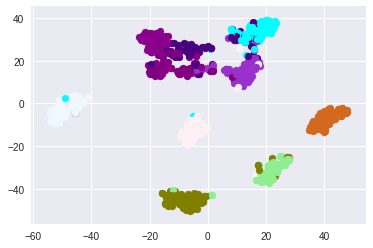
\includegraphics[width=\linewidth]{../output_plots/FMNIST/clustering/class-distribution-20.png}
	\caption{20\% training data classes}\label{fig:part_1_task_5_class_20}
	\endminipage\\
	\minipage{0.33\textwidth}
	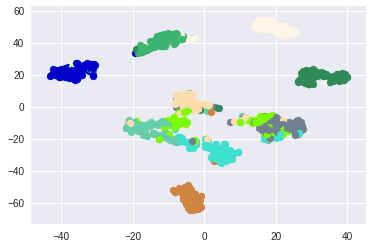
\includegraphics[width=\linewidth]{../output_plots/FMNIST/clustering/class-distribution-30.png}
	\caption{30\% training data classes}\label{fig:part_1_task_5_class_30}
	\endminipage\hfill
	\minipage{0.33\textwidth}
	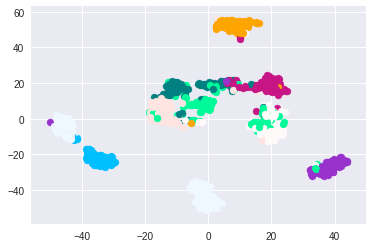
\includegraphics[width=\linewidth]{../output_plots/FMNIST/clustering/class-distribution-40.png}
	\caption{40\% training data classes}\label{fig:part_1_task_5_class_40}
	\endminipage
	\minipage{0.33\textwidth}
	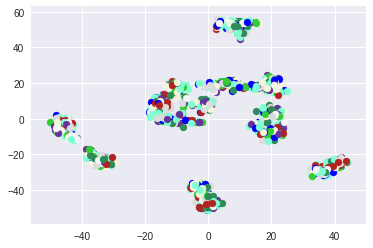
\includegraphics[width=\linewidth]{../output_plots/FMNIST/clustering/class-distribution-50.png}
	\caption{50\% training data classes}\label{fig:part_1_task_5_class_50}
	\endminipage
\end{figure}

\pagebreak
\subsection{Task 7: MLP vs CNN}
Trained model on a simple MLP consisting of 512 and 192 hidden layer nodes in two layers. The plots of various evaluation metrics are as follows:

\begin{figure}[!htb]
	\minipage{0.33\textwidth}
	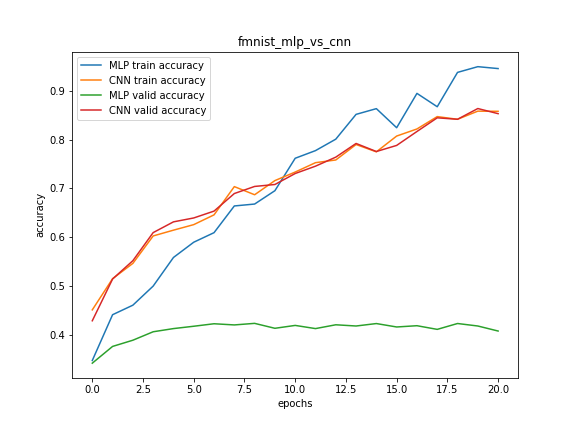
\includegraphics[width=\linewidth]{../output_plots/FMNIST/task-7/fmnist-mlp-vs-cnn-Accuracy-accuracy.png}
	\caption{Accuracy}\label{fig:part_1_task_7_accuracy}
	\endminipage\hfill
	\minipage{0.33\textwidth}
	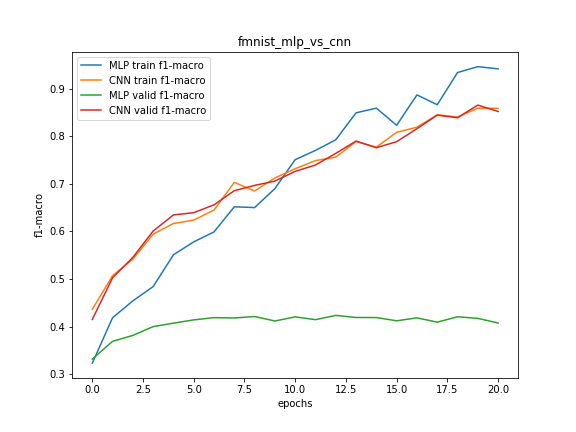
\includegraphics[width=\linewidth]{../output_plots/FMNIST/task-7/fmnist-mlp-vs-cnn-F1-Macro-score-f1-macro.png}
	\caption{F1-Micro}\label{fig:part_1_task_7_f1-micro}
	\endminipage
	\minipage{0.33\textwidth}
	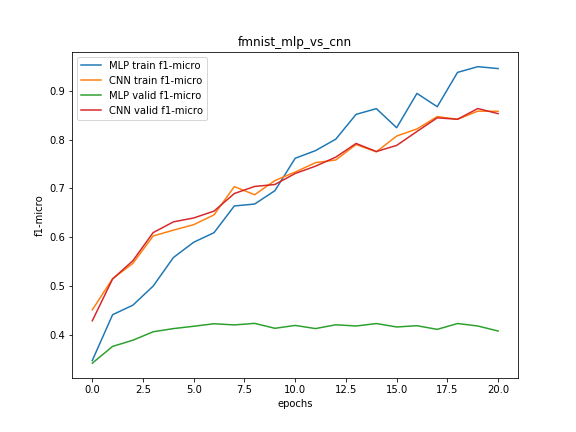
\includegraphics[width=\linewidth]{../output_plots/FMNIST/task-7/fmnist-mlp-vs-cnn-F1-Micro-score-f1-micro.png}
	\caption{F1-Macro}\label{fig:part_1_task_7_f1-macro}
	\endminipage
\end{figure}

\pagebreak
\section{Part 2:- CIFAR}
\subsection{Task 1:- Test Model with different number of layers}
Tested model with following architectures:
\begin{itemize}
	\item conv-3-3-64-fcn-100-10
	\item conv-5-5-32-conv-3-3-64-fcn-100-10
	\item conv-5-5-64-fcn-384-192-10
\end{itemize}

\begin{figure}[!htb]
	\minipage{0.33\textwidth}
	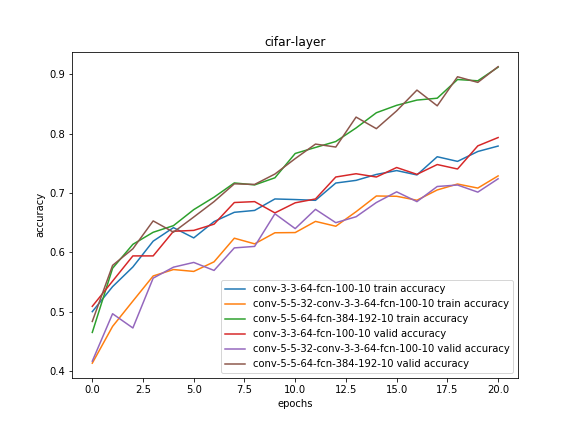
\includegraphics[width=\linewidth]{../output_plots/CIFAR/task-1/cifar-layer-Accuracy-accuracy.png}
	\caption{Accuracy}\label{fig:part_2_task_1_accuracy}
	\endminipage\hfill
	\minipage{0.33\textwidth}%
	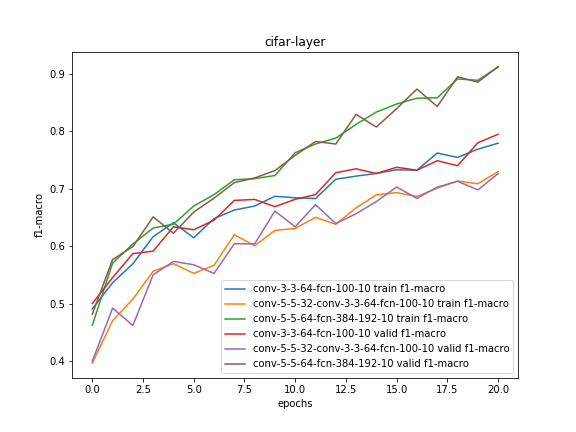
\includegraphics[width=\linewidth]{../output_plots/CIFAR/task-1/cifar-layer-F1-macro-score-f1-macro.png}
	\caption{F1-Micro}\label{fig:part_2_task_1_f1-micro}
	\endminipage
	\minipage{0.33\textwidth}%
	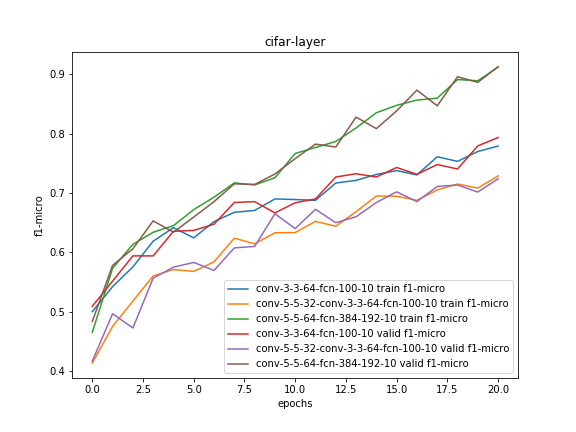
\includegraphics[width=\linewidth]{../output_plots/CIFAR/task-1/cifar-layer-F1-micro-score-f1-micro.png}
	\caption{F1-Macro}\label{fig:part_2_task_1_f1-macro}
	\endminipage
\end{figure}

Each plot shows the metric on Y-axis and epochs on X-axis. Different lines in plot corresponds to different models.

\subsection{Task 2:- Test Model with different number of neurons and layers}

Tested model with following configurations:
\begin{itemize}
	\item conv-5-5-32-conv-3-3-64-fcn-300-100-10
	\item conv-5-5-32-conv-5-5-32-fcn-200-50-10
	\item conv-5-5-64-conv-3-3-64-fcn-100-50-10
\end{itemize}

Finally fixed and fine-tuned the 784-50-30-10 model as it took less time for training and had comparable performance.

\begin{figure}[!htb]
	\minipage{0.33\textwidth}
	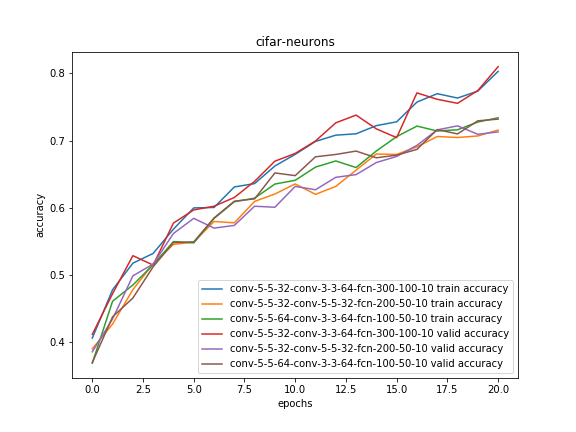
\includegraphics[width=\linewidth]{../output_plots/CIFAR/task-2/cifar-neurons-Accuracy-accuracy.png}
	\caption{Accuracy}\label{fig:part_2_task_2_accuracy}
	\endminipage\hfill
	\minipage{0.33\textwidth}%
	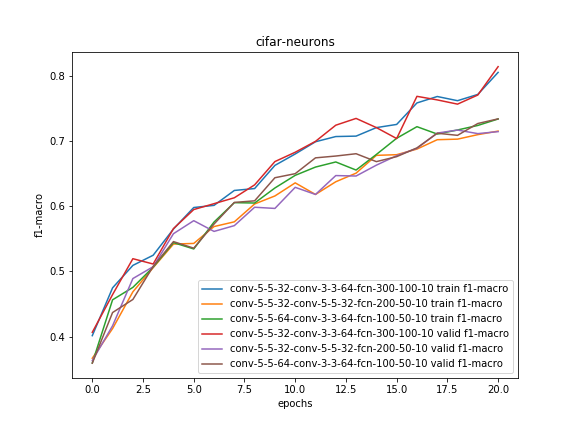
\includegraphics[width=\linewidth]{../output_plots/CIFAR/task-2/cifar-neurons-F1-macro-score-f1-macro.png}
	\caption{F1-Micro}\label{fig:part_2_task_2_f1-micro}
	\endminipage
	\minipage{0.33\textwidth}%
	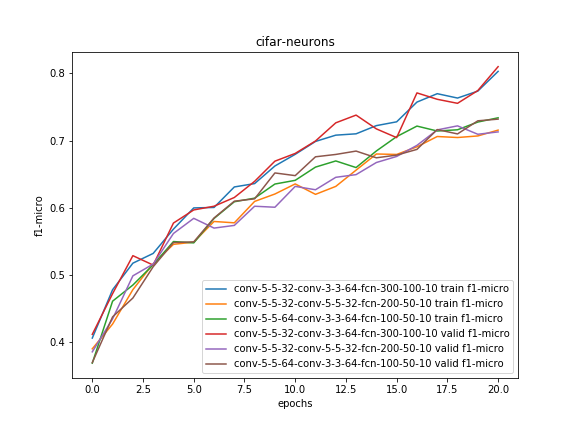
\includegraphics[width=\linewidth]{../output_plots/CIFAR/task-2/cifar-neurons-F1-micro-score-f1-micro.png}
	\caption{F1-Macro}\label{fig:part_2_task_2_f1-macro}
	\endminipage
\end{figure}

Each plot shows the metric on Y-axis and epochs on X-axis. Different lines in plot corresponds to different models.

\subsection{Task 3:- Test Model with different activation functions}

Tested model with relu, tanh, sigmoid and swish activations functions. The performance of relu and swish were almost same and decided to use swish in the final model.

\begin{figure}[!htb]
	\minipage{0.33\textwidth}
	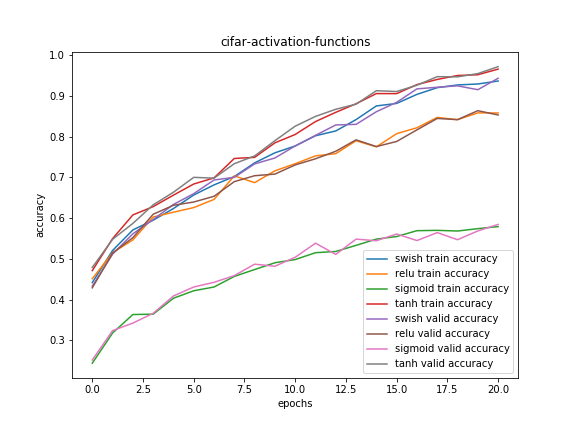
\includegraphics[width=\linewidth]{../output_plots/CIFAR/task-3/cifar-activation-functions-Accuracy-accuracy.png}
	\caption{Accuracy}\label{fig:part_2_task_3_accuracy}
	\endminipage\hfill
	\minipage{0.33\textwidth}
	\includegraphics[width=\linewidth]{../output_plots/CIFAR/task-3/cifar-activation-functions-F1-Macro-score-f1-macro.png}
	\caption{F1-Micro}\label{fig:part_2_task_3_f1-micro}
	\endminipage
	\minipage{0.33\textwidth}
	\includegraphics[width=\linewidth]{../output_plots/CIFAR/task-3/cifar-activation-functions-F1-Micro-score-f1-micro.png}
	\caption{F1-Macro}\label{fig:part_2_task_3_f1-macro}
	\endminipage
\end{figure}

Each plot shows the metric on Y-axis and epochs on X-axis. Different lines in plot corresponds to different models.

\pagebreak
\subsection{Task 4}
After observing above results and trying out various initialization techniques following architecture was finalized:
\begin{enumerate}
	\item Conv1: filter=5x5x3x64, activation=relu
	\item MaxPool1: kernel=2x2, strides=3x3
	\item Conv2: filter=3x3x64x64, activation=relu
	\item MaxPool2: kernel=2x2, strides=3x3
	\item FCN1: output=384, activation=relu
	\item FCN2: output=192, activation=relu
	\item Final output using softmax.
\end{enumerate}

\subsection{Task 5: Semi-supervised learning}
In this task model (selected in Task 4) was trained on 10-50\% of the data and embedding for rest of the images were extracted from the final layer just before the output layer of the network. The images were then clustered according to these embedding into 15 clusters and each cluster was assigned a class label depending on the highest number of images into that cluster belonging to same class.

The final accuracy achieved on validation set after taking 10-50\% of training data in increments of 10\% is as below:
\begin{table}[!htb]
	\centering
	\begin{tabular}{|c|c|}
		\hline
		Training instances & Accuracy\\
		\hline
		10\% & 39.7\%\\
		20\% & 42.3\%\\
		30\% & 48.5\%\\
		40\% & 49.7\%\\
		50\% & 58.4\%\\
		\hline
	\end{tabular}
\end{table}\\

\subsection{Task 6:- Cluster Projection}
The graphs obtained from above configuration of training instances is as below. These graphs were generated by projecting 1000 randomly selected instances into 2D using t-SNE projection method.

\begin{figure}[!htb]
	\minipage{0.5\textwidth}
	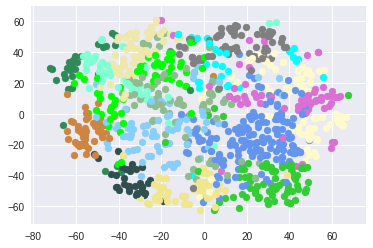
\includegraphics[width=\linewidth]{../output_plots/CIFAR/clustering/clusters-distribution-10.png}
	\caption{10\% training data clusters}\label{fig:part_2_task_5_cluster_10}
	\endminipage\hfill
	\minipage{0.5\textwidth}
	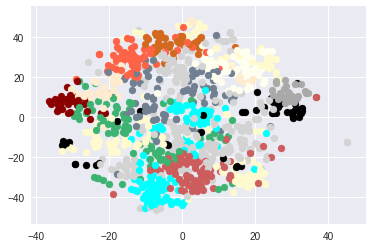
\includegraphics[width=\linewidth]{../output_plots/CIFAR/clustering/cluster-dstribution-20.png}
	\caption{20\% training data clusters}\label{fig:part_2_task_5_cluster_20}
	\endminipage\\
	\minipage{0.33\textwidth}
	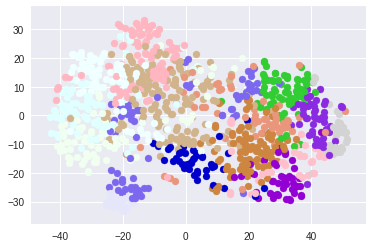
\includegraphics[width=\linewidth]{../output_plots/CIFAR/clustering/cluster-dstribution-30.png}
	\caption{30\% training data clusters}\label{fig:part_2_task_5_cluster_30}
	\endminipage\hfill
	\minipage{0.33\textwidth}
	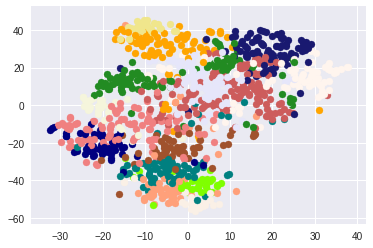
\includegraphics[width=\linewidth]{../output_plots/CIFAR/clustering/cluster-dstribution-40.png}
	\caption{40\% training data clusters}\label{fig:part_2_task_5_cluster_40}
	\endminipage
	\minipage{0.33\textwidth}
	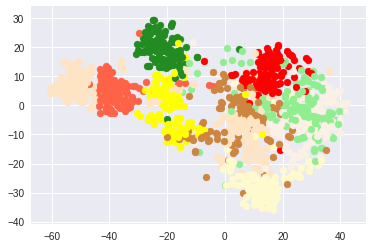
\includegraphics[width=\linewidth]{../output_plots/CIFAR/clustering/cluster-dstribution-50.png}
	\caption{50\% training data clusters}\label{fig:part_2_task_5_cluster_50}
	\endminipage
\end{figure}

The corresponding class distribution of points is as below:
\begin{figure}[!htb]
	\minipage{0.5\textwidth}
	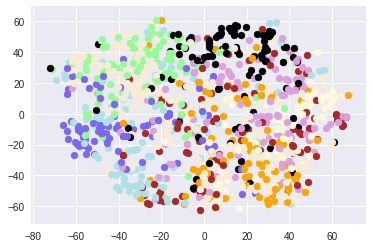
\includegraphics[width=\linewidth]{../output_plots/CIFAR/clustering/class-dstribution-10.png}
	\caption{10\% training data classes}\label{fig:part_2_task_5_class_10}
	\endminipage\hfill
	\minipage{0.5\textwidth}
	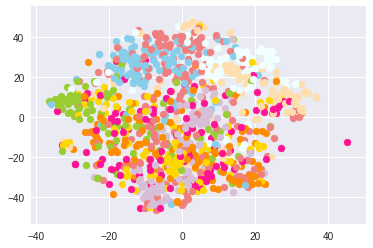
\includegraphics[width=\linewidth]{../output_plots/CIFAR/clustering/class-dstribution-20.png}
	\caption{20\% training data classes}\label{fig:part_2_task_5_class_20}
	\endminipage\\
	\minipage{0.33\textwidth}
	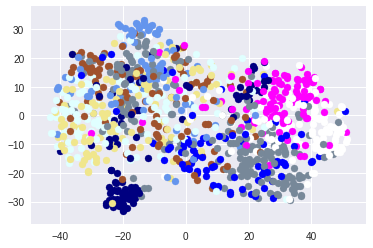
\includegraphics[width=\linewidth]{../output_plots/CIFAR/clustering/class-dstribution-30.png}
	\caption{30\% training data classes}\label{fig:part_2_task_5_class_30}
	\endminipage\hfill
	\minipage{0.33\textwidth}
	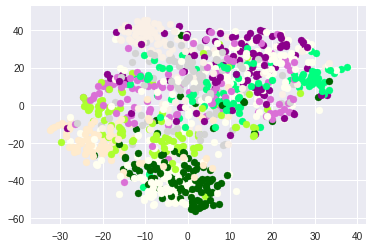
\includegraphics[width=\linewidth]{../output_plots/CIFAR/clustering/class-dstribution-40.png}
	\caption{40\% training data classes}\label{fig:part_2_task_5_class_40}
	\endminipage
	\minipage{0.33\textwidth}
	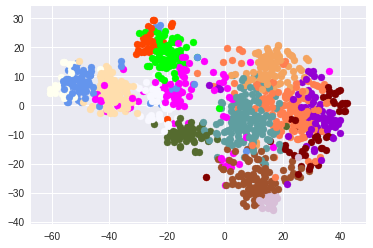
\includegraphics[width=\linewidth]{../output_plots/CIFAR/clustering/class-dstribution-50.png}
	\caption{50\% training data classes}\label{fig:part_2_task_5_class_50}
	\endminipage
\end{figure}

\pagebreak
\subsection{Task 7: MLP vs CNN}
Trained model on a simple MLP consisting of 512 and 192 hidden layer nodes in two layers. The plots of various evaluation metrics are as follows:

\begin{figure}[!htb]
	\minipage{0.33\textwidth}
	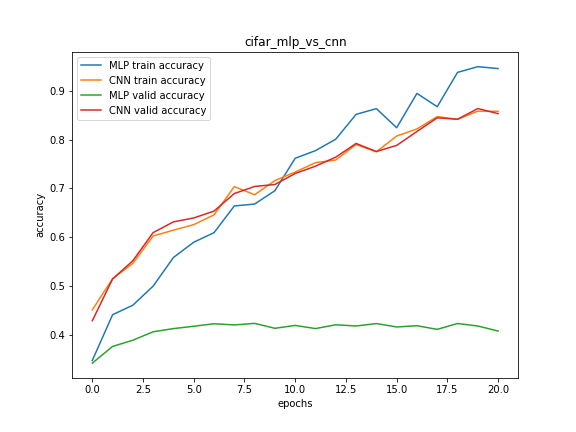
\includegraphics[width=\linewidth]{../output_plots/CIFAR/task-7/cifar-mlp-vs-cnn-Accuracy-accuracy.png}
	\caption{Accuracy}\label{fig:part_2_task_7_accuracy}
	\endminipage\hfill
	\minipage{0.33\textwidth}
	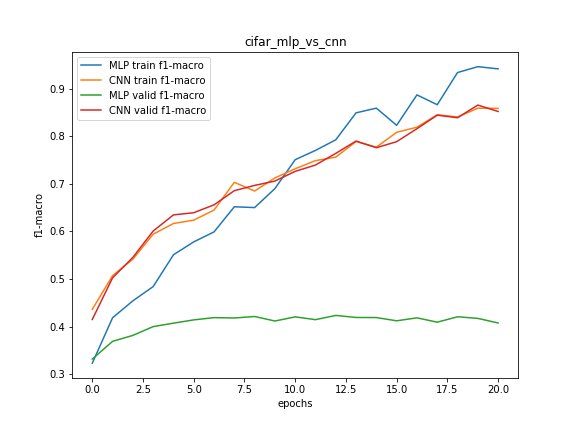
\includegraphics[width=\linewidth]{../output_plots/CIFAR/task-7/cifar-mlp-vs-cnn-F1-Macro-score-f1-macro.png}
	\caption{F1-Micro}\label{fig:part_2_task_7_f1-micro}
	\endminipage
	\minipage{0.33\textwidth}
	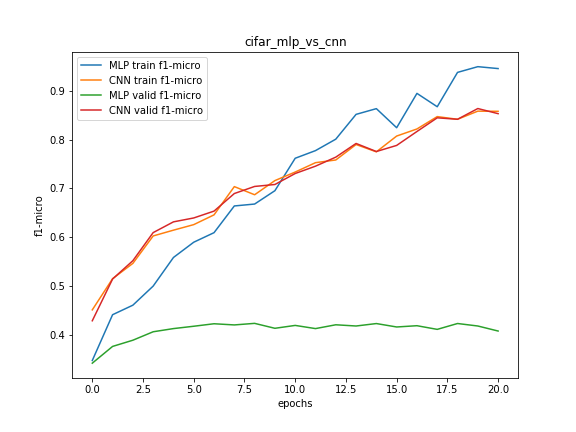
\includegraphics[width=\linewidth]{../output_plots/CIFAR/task-7/cifar-mlp-vs-cnn-F1-Micro-score-f1-micro.png}
	\caption{F1-Macro}\label{fig:part_2_task_7_f1-macro}
	\endminipage
\end{figure}


\end{document}